% HQIV: light-cone-derived auxiliary fields and sparse simulation
% Companion narrative to Lean modules (see HQIVLEAN.lean import closure):
%   Hqiv/Geometry/{OctonionicLightCone,AlphaGammaForcedByLattice,AuxiliaryFieldSmeared,ContinuumSpacetimeChart,ContinuumMetricGradient}.lean
%   Hqiv/Algebra/OctonionBasics.lean
%   Hqiv/QuantumComputing/{DiscreteQuantumState,DigitalGates,DigitalQuantumSimulation,OctonionicFT,OSHoracle,SparseSimulationDensityCrossover,OSHoracleHQIVNative,ProteinFoldingHook}.lean
%   Hqiv/Physics/{Action,ActionPlasmaBridge,LightConeMaxwellQFTBridge,ContinuumOmaxwellClosure}.lean
%   Hqiv/QuantumMechanics/{Schrodinger,AuxFieldBellDelayedChoice,BornMeasurementFinite,BornRuleFirstPrinciples,BornGleasonDecisionScaffold,
%     HorizonLimitedQM_QFT_Closure,HorizonLimitedRenormLocality,ContinuumManyBodyQFTScaffold,
%     ContinuumManyBodyQFTClosureLink,PatchIntervalMaxSmeared}.lean
%   Hqiv/Physics/CMBBirefringenceFirstPrinciples.lean (theory-only $\beta_{\mathrm{rad}}$ hook from $\alpha$, \texttt{referenceM})
%   Hqiv/Physics/SpinStatistics.lean (constructive spin--statistics slot for the continuum bundle)
%   Hqiv/ProteinResearch/{AtomEnergyOSHoracleBridge,ProteinFoldingQuantumChemistry,ProteinQCRefinement,AdditiveFieldAndTorque}.lean

\documentclass[11pt,a4paper]{article}

\usepackage{amsmath,amssymb,amsthm,mathtools}
\usepackage{microtype}
\usepackage[hidelinks]{hyperref}
\usepackage{xurl}
\newcommand{\lean}[1]{\path{#1}}
\usepackage[margin=1in]{geometry}
\usepackage{tikz}
\usetikzlibrary{arrows.meta,positioning}
\usepackage{array}
\usepackage[most]{tcolorbox}
\setlength{\emergencystretch}{3em}

\newtcolorbox{formalbox}{
  colback=blue!4!white,
  colframe=blue!45!black,
  boxrule=0.4pt,
  arc=2pt,
  left=6pt,right=6pt,top=4pt,bottom=4pt,
  fonttitle=\bfseries\small,
  title={Formal (Lean theorem / definition)},
}
\newtcolorbox{interpbox}{
  colback=orange!4!white,
  colframe=orange!55!black,
  boxrule=0.4pt,
  arc=2pt,
  left=6pt,right=6pt,top=4pt,bottom=4pt,
  fonttitle=\bfseries\small,
  title={Interpretive (physics narrative; not a standalone Lean theorem)},
}

\theoremstyle{remark}
\newtheorem{remark}{Remark}

\title{Light-Cone-Derived Auxiliary Fields Supply an Explicit Derived Interpretation of Quantum Superposition:\\Octonionic States, Lossless Bookkeeping, and Practical Sparse Simulation}
\author{Steven Ettinger Jr}
\date{\today}

\begin{document}
\maketitle

\begin{abstract}
This manuscript presents a Lean-aligned derivation showing that an auxiliary field and rapidity ladder induced directly from discrete null-lattice light-cone combinatorics supply an explicit, lossless interpretation of quantum superposition on an octonionic $\mathbb{R}^8$ carrier, while simultaneously reproducing inner-product invariants of standard quantum mechanics and enabling an exact sparse horizon-causal update rule for efficient classical simulation in structured regimes. \textbf{QM/QFT bridge (horizon-limited):} the library now packages a finite measurement layer with Born normalization, stochastic-kernel composition, and closed energy ledgers (auxiliary plus birefringence/redshift channels) in \lean{HorizonLimitedQM_QFT_Closure}, and combines it with a continuum closure statement \lean{HorizonContinuumClosureStatementCoreHQIV}: spin--statistics is discharged constructively (\texttt{SpinStatistics}), the finite classical CPTP/Markov slot is discharged (\lean{cptp_density_closure_finite_classical_holds}), and the shell-to-harmonic ratio bridge plus microcausality scaffolding (lattice, Minkowski, or interval-max surrogates) are wired through \lean{HorizonLimitedRenormLocality} and \lean{ContinuumManyBodyQFTClosureLink}, with an operator-layer commutator companion in \texttt{PatchIntervalMaxSmeared}. Renormalization-, cluster-, and scattering-consistency fields are currently instantiated by explicit \emph{scaffold} witnesses (documented in Lean as placeholders rather than full interacting many-body QFT theorems). \textbf{IR/UV:} the discrete carrier is ultraviolet-finite by construction; infrared structure is horizon-limited (narrative cutoff) with convex smearing of $\phi$ along shells (\texttt{AuxiliaryFieldSmeared}). \textbf{Measurement problem (auxiliary-carrier paradigm):} the auxiliary field and horizon-limited light-cone structure supply \emph{full local bookkeeping} of energy flows and probability currents within the causal patch. Lean discharges the finite layer: \texttt{AuxFieldBellDelayedChoice} and \texttt{BornMeasurementFinite} prove that linear calibrated maps cannot yield definite single outcomes from nontrivial superpositions; ledger theorems close apparent flows through auxiliary and birefringence/redshift channels with Born-\emph{consistent} finite channels (\lean{HorizonLimitedQM_QFT_Closure}). \textbf{Interpretive stance:} deterministic local accounting excludes \textbf{globally branching} many-worlds readings; the algebraic foundation aligns with a \textbf{pilot-wave} ontology in which measurement \textbf{selection} is an explicit, calibrated map enforcing Born statistics \textbf{without} stochastic dynamical collapse (GRW/Penrose). At the finite level, \texttt{BornRuleFirstPrinciples} \textbf{forces} uniqueness: coherent amplitude--square weights (\texttt{BornCoherent}) \emph{coincide} with Born ratios in \texttt{BornMeasurementFinite} (\lean{bornProbN_unique_of_coherence}); \lean{BornGleasonDecisionScaffold} records extension to a Gleason-style axiom bundle. The preferred-basis problem is not claimed solved in full generality. The construction is a \textbf{representation-level reformulation} focused on operational completeness and conservation. \textbf{Discrete forcing:} the shell-wise curvature-imprint ratio \texttt{latticeAlphaRatio} equals $\alpha$ for every $n$ and evaluates to $3/5$ (\lean{latticeAlphaRatio_eq_alpha}, \texttt{alpha\_eq\_3\_5}); the unit horizon split \texttt{gamma\_HQIV}$:=1-\alpha$ \textbf{forces} $\gamma=2/5$ (\texttt{gamma\_eq\_2\_5}), jointly packaged as \lean{alpha_gamma_forced_pair} in \texttt{AlphaGammaForcedByLattice}. Companion HQIV theory \cite{ettinger2026hqiv,brodie2026} supplies the physical thermodynamic and geometric narrative; Lean \textbf{discharges uniqueness} of the displayed rationals from the discrete definitions. \textbf{Cosmic-scale auxiliary channel:} the same birefringence bookkeeping used in the measurement layer is the formal home of polarization-rotation observables; companion HQIV work ties this to measurable $\beta$ at CMB scales \cite{ettinger2026hqiv}. Lean also packages a \textbf{theory-only} angle \lean{betaRad_HQIV_imprint} and redshift identity \lean{one_add_birefringence_HQIV_imprint} in \lean{CMBBirefringenceFirstPrinciples} (from $\alpha$ and \texttt{referenceM}, without importing an experimental $\beta$). \textbf{Thermodynamic and vacuum-sector displays:} shell thermodynamics $T(m)$, composite curvature norm $\mathcal{N}_{\mathrm{curv}}$, and related companion targets are \textbf{derived in the companion HQIV manuscript} \cite{ettinger2026hqiv}; here $\alpha$ and $\gamma$ are \textbf{not} free parameters---they are \textbf{forced} in Lean as above, while this paper shows sparse simulation and operational embedding. \textbf{Protein / quantum chemistry:} Lean proves nonnegative traceable site-energy contracts and QC-refinement descent algebra (\lean{ProteinFoldingQuantumChemistry}, \texttt{ProteinQCRefinement}, \texttt{AtomEnergyOSHoracleBridge}); sparse HQIV-native gates appear in \texttt{ProteinFoldingHook}/\texttt{OSHoracleHQIVNative}. Companion Python pipelines that implement the same contracts have been exercised on CAMEO-class design targets with reported agreement against experimental reference data---those numerical comparisons lie outside the Lean proof corpus. Beyond the measurement paradigm stated above, the manuscript does not claim modifications to QM observables except through the stated bookkeeping channels.
\end{abstract}

\medskip
\noindent\textbf{Repository.} \url{https://github.com/disregardfiat/hqiv-lean}
\par\noindent\textbf{External protein pipeline.} \url{https://github.com/disregardfiat/PROtein_folder} (HQIV-aligned Python implementation; Lean contracts in \lean{Hqiv/ProteinResearch/})
\par\noindent\textbf{Versioned environment.} Lean 4.28.0 development context; companion archive DOI: \url{https://doi.org/10.5281/zenodo.18899939}

\noindent\textbf{Companion HQIV manuscript.} \cite{ettinger2026hqiv}

\paragraph{Reader guide: four layers of claim status.}
To keep formal traceability aligned with what is actually proved in Lean versus what is modeling convention or external numerics, read the manuscript through four layers: \textbf{(i)~Lean finite layer:} digital states, inner products, selected gates, measurement bookkeeping with explicit selection and closed ledgers, finite Born and stochastic-kernel closure (\lean{HorizonLimitedQM_QFT_Closure}), Born-weight uniqueness from coherence (\texttt{BornRuleFirstPrinciples}: \lean{bornProbN_unique_of_coherence}), and explicit algebraic lemmas (Bell/eraser identities, CHSH proxy arithmetic) in the cited modules. The \textbf{measurement-problem stance} is auxiliary-mediated local accounting (energy and probability currents), horizon-limited causality, pilot-wave--style ontology with a calibrated selection rule, Born without dynamical collapse, and rejection of globally branching many-worlds \emph{within this formalism}. \textbf{(ii)~Imported algebra:} octonion left-multiplication matrices and SO(8) scaffold are standard algebraic inputs, not derived from the three light-cone axioms alone. \textbf{(iii)~Companion HQIV physics:} \emph{derivation of the physical constants and vacuum-sector structure}---including the \textbf{unique} curvature-imprint exponent $\alpha=3/5$ and the \textbf{unique} monogamy coefficient $\gamma=2/5$ (with $\alpha+\gamma=1$ on the unit horizon split), shell thermodynamics $T(m)\propto 1/(m+1)$, composite curvature norm $\mathcal{N}_{\mathrm{curv}}$, and the informational-energy ladder---is carried out in \cite{ettinger2026hqiv} (with inertia/GR companions in \cite{brodie2026}). Those are \emph{the} HQIV $\alpha$ and $\gamma$, not a family of tunable alternatives; Lean exposes them only as \texttt{alpha} and \texttt{gamma\_HQIV} with proved rational identities. This preprint is the Lean-aligned \emph{compression} of that program into digital states, measurement ledgers, and sparse simulation; where the text speaks of ``normalization choices'' in a discrete ratio, the reader should read them as the discrete shadows of the companion derivation unless noted as purely representational. \textbf{(iv)~Continuum, phenomenology, and external validation:} horizon-limited continuum closure is now available as a proved theorem bundle \lean{HorizonContinuumClosureStatementCoreHQIV} assembled in \lean{HorizonLimitedRenormLocality} (via \lean{continuum_many_body_closure_*}) from minimal continuum fields plus constructive discharges for spin--statistics and finite classical CPTP; the remaining honesty boundary is that renormalization-, cluster-, and scattering-consistency slots use structured \emph{scaffold} witnesses until stronger interacting-QFT lemmas replace them. The CMB paragraph below \emph{imports} published $\beta$ as a consistency check; \lean{CMBBirefringenceFirstPrinciples} separately records a discrete-HQIV theory hook $(1+z)=\exp(\beta/\kappa)=(\texttt{referenceM}+1)^\alpha$ at $\kappa_\beta=1$---comparing that prediction to the measured $\beta$ distribution remains phenomenology outside Lean. Protein/CAMEO-class numerical agreement is reported from companion Python runs aligned to the Lean energy contracts, not as a formal theorem. \textbf{Forced uniqueness (discrete + metric):} once the cumulative simplex normalization and hockey-stick identity are in the formalism, \lean{latticeAlphaRatio_eq_alpha} gives $\alpha=3/5$ at every shell, and \texttt{gamma\_HQIV}$:=1-\alpha$ gives $\gamma=2/5$ (\texttt{AlphaGammaForcedByLattice}); these are \textbf{not} a tunable $(\alpha,\gamma)$ family within the Lean layer. Companion HQIV theory \cite{ettinger2026hqiv,brodie2026} supplies the physical thermodynamic shell structure and broader vacuum-sector derivation; the octonion factor $8$ in Axiom~1 fixes the division-algebra carrier dimension for this manuscript's gate scaffold. Sections~\ref{sec:axioms}--\ref{sec:sparse-pipeline} are largely (i)--(ii); Section~\ref{sec:lagrangian} records the Lean \texttt{Action}/\texttt{Schrodinger} variational layer; Section~\ref{sec:closing} mixes (i) with (iii)--(iv). \textbf{Appendices:} companion Zenodo DOIs and repository layout (Appendix~\ref{app:companions}); expanded four-layer guide (Appendix~\ref{app:fourlayers}); glossary of Lean identifiers (Appendix~\ref{app:glossary}); continuum/QFT proved vs.\ scaffold table (Appendix~\ref{app:qftbridge}); one-page roadmap figure (Appendix~\ref{app:roadmap}).

%--------------------------------------------------------------------
\section{Minimal light-cone axioms and the induced auxiliary-field bridge to digital quantum states}
\label{sec:axioms}

This manuscript is structured as a derivation from three core inputs, each mirrored by a dedicated Lean module:

\paragraph{Motivation: why light-cone discretization and why octonions.}
The starting point is an observer-centric past light-cone discretization because horizon thermodynamic and causal arguments naturally organize information by null-accessible shells \cite{jacobson1995,bombelli1987}. The shell-wise bookkeeping is then coupled to holographic-style information accounting \cite{susskind1994,bousso2002}. The octonionic factor $8$ is used because the carrier is explicitly $\mathbb{R}^8$ with seven imaginary directions supporting the non-associative division-algebra structure used in the gate scaffold; in this manuscript, $8$ is therefore not an arbitrary multiplier but the chosen algebraic carrier dimension \cite{baez2002octonions,freedman2019}. The companion HQIV line of work provides the broader geometric/physical context for this choice, including thermodynamic horizon-based inertia/GR-side derivations in companion materials \cite{ettinger2026hqiv,brodie2026}.

\paragraph{Axiomatic representation stance.}
In this work, the cosmic horizon (or, locally, an accelerated Rindler horizon) is treated as the natural infrared cutoff of the model. \textbf{Canonical constants.} In the companion HQIV program, the curvature-imprint exponent is \textbf{uniquely} $\alpha=3/5$ and the monogamy split is \textbf{uniquely} $\gamma=2/5$ (with $\alpha+\gamma=1$); their physical role and thermodynamic narrative are given in \cite{ettinger2026hqiv,brodie2026}. In Lean, \textbf{uniqueness is forced}: \lean{latticeAlphaRatio_eq_alpha} identifies the shell-wise curvature-imprint ratio with $\alpha$ at every $n$, and \texttt{alpha\_eq\_3\_5} evaluates $\alpha=3/5$; \texttt{gamma\_HQIV} is \emph{defined} as $1-\alpha$, so \texttt{gamma\_eq\_2\_5} is not an independent knob. These are packaged in \texttt{AlphaGammaForcedByLattice} (\lean{alpha_gamma_forced_pair}). Under the representation stance, the "$3$D null-lattice + octonion-$8$" axiom fixes the carrier and mode count; the companion manuscripts supply the geometric/thermodynamic \emph{derivation} of the HQIV vacuum sector, while this preprint and Lean \textbf{prove} the rational $(\alpha,\gamma)$ identities and their joint uniqueness from the discrete definitions together with the complement split. \emph{Remark:} a different algebraic carrier than octonion-$\mathbb{R}^8$ would define a different gate scaffold; this manuscript fixes the division-algebra $8$-dimensional carrier in Axiom~1.

\paragraph{Axiom 1 (Lightcone with octonionic degrees of freedom).}
At each discrete radial step $m$ on the observer past light-cone, the newly available horizon modes are governed by a single combinatorial rule:
the $3$D null-lattice stars-and-bars count for $x+y+z=m$ is multiplied by the octonion factor $8$.
In Lean, this appears as the light-cone mode axiom defining \lean{available_modes} and \texttt{new\_modes} in \lean{Hqiv/Geometry/OctonionicLightCone}.
After the fixed normalization conventions, this yields the working shell formulas used throughout the paper:
\[
  A(m) = 8\dbinom{m+2}{2} = 4(m+2)(m+1),
\]
and the per-shell incremental growth $\Delta A(m+1)=8(m+2)$.

\paragraph{Axiom 2 (Monogamy / CKW baseline).}
For three-party tangles, we start from the standard CKW-form monogamy constraint \cite{ckw2000}
\[
  \tau_{AB}+\tau_{AC}\le \tau_{A|BC}.
\]
\emph{Algebraic remark.} Multiplying this inequality by a fixed positive shell weight $\eta_{\phi}(m)>0$ yields an equivalent inequality in the same tangle variables; it does not, by itself, strengthen the logical content of CKW. The HQIV use of $\eta_{\mathrm{mode}}$ and $\eta_{\phi}$ is therefore a \emph{bookkeeping and normalization convention}: it tracks how discrete light-cone mode growth and the auxiliary $\phi$-ladder assign shell-dependent weights when \emph{stating} or \emph{comparing} inequalities across shells in the Lean development, and it aligns those weights with the same combinatorial ladder as Axiom~1.
In Lean, this is expressed via \texttt{etaMode} and \texttt{phi\_of\_shell} in \lean{Hqiv/QuantumMechanics/MonogamyTangles}.
\[
  \eta_{\mathrm{mode}}(m)=\frac{\text{new\_modes}(m)}{\text{available\_modes}(\text{referenceM})},
  \qquad
  \eta_{\phi}(m)=\frac{\eta_{\mathrm{mode}}(m)}{\phi(m)},
\]
and the $\eta_{\phi}$-weighted display
\[
  \eta_{\phi}(m)\tau_{AB}+\eta_{\phi}(m)\tau_{AC}\le \eta_{\phi}(m)\tau_{A|BC}
\]
is the same constraint after dividing by $\eta_{\phi}(m)$. Where Lean uses \emph{effective} quantities (e.g.\ $\eta$-scaled tangles) the module names make that role explicit.

\paragraph{Axiom 3 (Starting informational energy = 1).}
Digital states live on a finite angular ladder with an octonion Euclidean inner product per ladder slot.
The foundational normalization is that the informational-energy norm of a state equals one:
\[
  \|f\|^2 \;=\; \sum_{ij\in\mathcal{H}_L}\langle f(ij),f(ij)\rangle \;=\; 1.
\]
In Lean, this is encoded as the predicate \texttt{IsNormalized} in the
\texttt{DiscreteQuantumState} module.
This normalization is the condition that makes admissible digital evolutions behave as norm-preserving (unitary-style) operators on the finite model.

\paragraph{Roadmap.}
From these axioms, the derivation proceeds in the same order as the remaining sections:
\begin{enumerate}
  \item Lightcone mode axiom $\Rightarrow$ shell combinatorics $\Rightarrow$ curvature-imprint normalization and auxiliary-field/rapidity ladder.
  \item Lightcone mode weights $\Rightarrow$ shell factors (including the monogamy correction $\eta$ and its $\phi$-augmented form).
  \item Starting-energy normalization $\Rightarrow$ consistent superposition interpretation on the $\mathbb{R}^8$ octonionic carrier.
  \item Octonion left-multiplication $\Rightarrow$ algebraic gate scaffolding.
  \item Sparse horizon-causal register evolution $\Rightarrow$ expand/evolve/prune bookkeeping.
\end{enumerate}

%--------------------------------------------------------------------
\section{Discrete null lattice and mode counting}

\paragraph{Stars-and-bars on the $3$D null shell.}
At integer shell $m\ge 0$, count nonnegative integer triples $(x,y,z)$ with $x+y+z=m$. The textbook stars-and-bars cardinality is $\dbinom{m+2}{2}$. The Lean development tracks the numerator $(m+2)(m+1)$ and absorbs the factor $\tfrac12$ in related normalisations.

\begin{equation}
  N_{\mathrm{simp}}(m) \;=\; (m+2)(m+1).
\end{equation}

\paragraph{Cumulative shells.}
Summing through shell $n$ satisfies a hockey-stick identity that packages the binomial $\dbinom{n+3}{3}$:

\begin{equation}
  3\sum_{m=0}^{n} N_{\mathrm{simp}}(m) \;=\; (n+1)(n+2)(n+3),
  \qquad
  \sum_{m=0}^{n} N_{\mathrm{simp}}(m) \;=\; \frac{(n+1)(n+2)(n+3)}{3}.
\end{equation}

%--------------------------------------------------------------------
\section{Octonionic lift: available and new modes}

\paragraph{HQIV light-cone axiom (combinatorial).}
Newly available modes at shell $m$ combine the $3$D simplex count with an octonion factor $8$. Writing $C(m)=\dbinom{m+2}{2}=N_{\mathrm{simp}}(m)/2$,

\begin{equation}
  A(m) \;=\; 8\,C(m) \;=\; 4\,(m+2)(m+1).
\end{equation}

\paragraph{Incremental ``new modes''.}
For $m\ge 1$, the increment obeys a linear law in the formal development:

\begin{equation}
  \Delta A(m+1) \;=\; A(m+1)-A(m) \;=\; 8\,(m+2).
\end{equation}

%--------------------------------------------------------------------
\section{Lattice ratio and the curvature-imprint exponent}

\paragraph{Rational $\alpha$ from the ladder (normalization convention).}
Let $S(n)=\sum_{m\le n}N_{\mathrm{simp}}(m)$. The hockey-stick identity gives $(n+1)(n+2)(n+3)=3S(n)$. Define the shell-wise lattice ratio by
\begin{equation}
  r(n) \;=\; \frac{(n+1)(n+2)(n+3)}{5\,S(n)}.
\end{equation}
The factor $5$ in the denominator is \emph{not} forced by hockey-stick alone: in this manuscript it is the discrete \emph{display rule} that encodes the target curvature imprint exponent $\alpha=3/5$ into $r(n)$, since then $r(n)=3S(n)/(5S(n))=3/5$ for all $n$. In Lean, the proof is the same algebraic substitution. The \textbf{physical derivation} of the value $\alpha=3/5$ and its role in horizon-imprint/cosmology is given in the companion HQIV framework \cite{ettinger2026hqiv} and in \cite{brodie2026}; here $r(n)$ is the shell-by-shell rational bookkeeping that matches that fixed $\alpha$ in the discrete layer.

\paragraph{Per-shell curvature density and $\delta_E$.}
Sampling a continuous template at integer shells $x=m+1$,

\begin{equation}
  \rho(x) \;=\; \frac{1}{x}\Bigl(1+\alpha\ln x\Bigr),
  \qquad
  \sigma(m) \;=\; \rho(m+1) \;=\; \frac{1}{m+1}\Bigl(1+\alpha\ln(m+1)\Bigr).
\end{equation}

\paragraph{Combinatorial curvature norm (cube $\times$ octonion $\times$ geometry).}
Six directions from a $3$D cube ($\pm$ along each axis), raised to the $7$ imaginary octonion dimensions, times the half-diagonal $\sqrt{3}$ of the unit cube:

\begin{equation}
  \mathcal{N}_{\mathrm{curv}} \;=\; 6^{7}\sqrt{3} \;=\; 279\,936\,\sqrt{3}.
\end{equation}
This factor packages ``direction count'' $\times$ ``octonion-imaginary lift'' $\times$ ``rapidity geometric scale''. Its \textbf{geometric derivation} from the horizon--cube--octonion scaffold is part of the companion HQIV development \cite{ettinger2026hqiv}; in Lean it appears as the explicit composite $\mathcal{N}_{\mathrm{curv}}$ used consistently for $\delta_E$.

\paragraph{Per-shell imprint.}
\begin{equation}
  \delta_E(m) \;=\; \mathcal{N}_{\mathrm{curv}}\,\sigma(m).
\end{equation}

\paragraph{Horizon-dependent curvature ratio.}
For a reference horizon $N$ with positive partial integral $I(N)=\sum_{m<N}|\sigma(m)|$,

\begin{equation}
  \Omega_k(n;N) \;=\; \frac{I(n)}{I(N)} \quad\text{(when }I(N)>0\text{)}.
\end{equation}

%--------------------------------------------------------------------
\section{Octonions as \texorpdfstring{$\mathbb{R}^8$}{R8} with left-multiplication matrices}

\paragraph{Carrier and inner product.}
Octonions are realised as vectors $x\in\mathbb{R}^8\cong\mathrm{Fin}\,8\to\mathbb{R}$ with basis $e_0,\ldots,e_7$. Multiplication uses fixed left-multiplication matrices $L(e_i)$ (from the generator module). The Euclidean octonion inner product is

\begin{equation}
  \langle x,y\rangle \;=\; \sum_{k=0}^{7} x_k\,y_k.
\end{equation}

\paragraph{Norm preservation.}
Each nontrivial imaginary left multiplier $L(e_i)$ preserves the Euclidean sum of squares; $L(e_0)$ is the identity. This is the analytic backbone for octonion-valued digital amplitudes.

\paragraph{Non-associativity remark.}
Octonion non-associativity does not obstruct the finite gate layer used here because updates are implemented through fixed left-multiplication linear maps (matrices) composed as linear operators on the state carrier. In other words, associativity is required at the level of operator composition, not at the raw octonion product level; this is why norm-preserving gate construction can remain well-defined in the present scaffold \cite{baez2002octonions,freedman2019}.

\paragraph{Dependency boundary (important).}
The matrix identities for left multiplication are algebraic inputs from the octonion/Fano representation and do not require an auxiliary-field hypothesis to be stated. In the Lean stack, this is the role of `OctonionLeftMultiplication` and `OctonionBasics`. However, the \emph{physical weighting} attached to those carriers in HQIV evolution---shell factors, effective energy scales, and rapidity-linked curvature bookkeeping---does depend on the same light-cone-derived ladder that fixes the auxiliary field.

%--------------------------------------------------------------------
\section{Auxiliary field and rapidity derivation bridge}

\paragraph{Auxiliary field is derived, not fitted.}
The auxiliary field is tied to the shell temperature ladder:
\[
  T(m)=\frac{T_{\mathrm{Pl}}}{m+1},\qquad
  \phi(m)=\frac{2}{T(m)}=2(m+1),
\]
so once the discrete Planck-scale temperature profile $T(m)\propto 1/(m+1)$ is adopted, $\phi(m)=2(m+1)$ follows algebraically. That temperature law is \textbf{derived in the companion thermodynamic/informational treatment} of the HQIV vacuum \cite{ettinger2026hqiv}; it is not an independent continuous fit. This manuscript uses it as the same ladder as mode counting for structural consistency.

\paragraph{Rapidity/geometry factor in the same chain.}
The curvature-imprint normalization uses the formal geometric factor $6^7\sqrt{3}$, where $\sqrt{3}$ is the unit-cube half-diagonal (rapidity-lattice geometric contribution) and $6^7$ is the cube-direction/octet dimensional lift. This places auxiliary-field scaling and rapidity geometry in a single derivation path from the light-cone combinatorics.

\paragraph{Why this matters for sparse horizon-causal updates.}
Because carrier algebra (left multiplication), shell weighting ($\phi$ ladder), and curvature/rapidity normalization are sourced from one formal chain, sparse horizon-causal evolution is presented as exact model bookkeeping in the proved finite setting, not a heuristic shortcut.

%--------------------------------------------------------------------
\section{Digital quantum states on the angular ladder}

\paragraph{Harmonic index and dimension.}
Fix cutoff $L$. Angular indices are pairs $(\ell,\mu)$ with $\ell\in\{0,\ldots,L\}$ and magnetic index $\mu\in\{-\ell,\ldots,\ell\}$ ($2\ell+1$ values per $\ell$), matching spherical-harmonic degeneracy:

\begin{equation}
  |\mathcal{H}_L| \;=\; \sum_{\ell=0}^{L} (2\ell+1) \;=\; (L+1)^2.
\end{equation}
To avoid confusion with the \emph{radial shell index} $m$ on the null cone (Sections~\ref{sec:axioms}--\ref{sec:sparse-pipeline}), this section uses $\ell$ for the orbital label on the harmonic ladder and reserves $\mu$ for the magnetic index; the symbol $m$ always means ``radial shell'' outside this harmonic slot.

\paragraph{Rational temperature shadow.}
The rational ladder weight mirrors the continuous shell factor $\phi_{\mathrm{shell}}(m)=2(m+1)$ but is indexed by the slot's orbital label $\ell$:
\begin{equation}
  \phi_{\mathrm{rat}}(\ell) \;=\; 2(\ell+1)\in\mathbb{Q}.
\end{equation}
Thus $\phi_{\mathrm{rat}}(\ell)=2(\ell+1)$ is evaluated on nonnegative integers only; it is not the magnetic quantum number $\mu$.

\paragraph{State space and informational inner product.}
A digital state assigns an octonion $8$-vector to each harmonic slot (indexed by $(\ell,\mu)$ with $\mathcal{H}_L$ as above):

\begin{equation}
  f:\mathcal{H}_L \to \mathbb{R}^8,
  \qquad
  \langle\!\langle f,g\rangle\!\rangle \;=\; \sum_{(\ell,\mu)\in\mathcal{H}_L} \langle f(\ell,\mu),g(\ell,\mu)\rangle.
\end{equation}

\paragraph{Normalisation.}
$\|f\|^2=\langle\!\langle f,f\rangle\!\rangle$; ``physical'' digital kets satisfy $\|f\|^2=1$.

\paragraph{Correspondence back to standard complex-Hilbert bookkeeping.}
A practical embedding map is obtained by pairing real carrier components into complex amplitudes on each slot, e.g.
\[
  \Pi(f)(ij) = \bigl(f_0(ij)+i f_1(ij),\, f_2(ij)+i f_3(ij),\, f_4(ij)+i f_5(ij),\, f_6(ij)+i f_7(ij)\bigr)\in\mathbb{C}^4.
\]
Under this projection, the slotwise Euclidean norm equals the complex $\ell_2$ norm of the embedded amplitudes, so the global discrete norm induces standard finite-dimensional Hilbert bookkeeping. Mixed-state bookkeeping is then obtained in the usual way from projected pure states, $\rho=\sum_a p_a \left|\Pi(f_a)\right\rangle\!\left\langle\Pi(f_a)\right|$, so the finite octonionic carrier can be read as a real lift compatible with conventional density-operator practice \cite{vonNeumann1955,dirac1930}.

\paragraph{Small global example (entangled two-slot state).}
For two selected slots $s_0,s_1$, define projected amplitudes
\[
  \Pi(f)(s_0)=\frac{1}{\sqrt{2}}(1,0,0,0),\qquad
  \Pi(f)(s_1)=\frac{1}{\sqrt{2}}(0,1,0,0),
\]
with all other slots zero. This is the finite-ladder analogue of a Bell-like superposition in the projected complex model; norm preservation under admissible gates follows from the same inner-product invariants stated above.

%--------------------------------------------------------------------
\section{Digital gates and time evolution}
\label{sec:gates}

\paragraph{HQIV gate.}
A digital gate is an inner-product-preserving bijection $U$ acting on digital states $f:\mathcal{H}_L\to\mathbb{R}^8$, meaning it preserves the discrete informational inner product $\langle\!\langle\cdot,\cdot\rangle\!\rangle$. Equivalently on each slot, $U$ induces an orthogonal transformation of the eight real coordinates (a subgroup of $O(8)$ on the carrier), composed with slot permutations allowed by the scaffold. This is \emph{not} the most general unitary on the complex Hilbert space obtained after $\Pi$ unless one restricts further; the proved scope of this manuscript is a \emph{representation-level} real lift with prescribed invariants, not full equivalence to arbitrary $U(d)$ quantum circuits on the embedded complex space \cite{vonNeumann1955,dirac1930}. In orthodox quantum mechanics, norm-preserving evolution is represented by unitary operators; here admissible maps play the analogous bookkeeping role on the real octonionic carrier \cite{freedman2019}.

\paragraph{Examples in the scaffold.}
We illustrate the allowed gate primitives with four scaffold examples: phase flips on a single mode; swaps of modes sharing the same $\ell$ (so $\phi_{\mathrm{rat}}$ weighting is consistent across the swap); octonion left actions that preserve Euclidean octonion norm on each slot; and a finite $4$-point permutation representing a CNOT-type swap on a binary sub-register.

\paragraph{Hadamard shell identity (rational, no $\sqrt{2}$).}
On the two-dimensional rational subspace spanned by a pair of slots, the \emph{unnormalized} Hadamard linear map $H_{\mathrm{raw}}$ sends $(v_0,v_1)\mapsto(v_0+v_1,v_0-v_1)$. Writing $v=(v_0,v_1)\in\mathbb{Q}^2$,

\begin{equation}
  (v_0+v_1)^2 + (v_0-v_1)^2 \;=\; 2\,(v_0^2+v_1^2).
\end{equation}
This rational bookkeeping is the same technique used in exact-arithmetic quantum-circuit simulators to defer normalisation until the end of a gate sequence \cite{smith2019exact}.

This is the squared-norm relation for $H_{\mathrm{raw}}H_{\mathrm{raw}}^{\mathsf T}=2I$: it tracks an overall factor of $2$ in Euclidean energy, not strict norm preservation on the \emph{unnormalized} coordinates. The \emph{physical} admissible gate in the sense of the HQIV definition above is the orthogonal (norm-preserving) operator $\tfrac{1}{\sqrt{2}}H_{\mathrm{raw}}$, or equivalently the composition of $H_{\mathrm{raw}}$ with an explicit global renormalization step that restores $\|f\|^2=1$ on the full digital state; the rational scaffold keeps exact rationals by deferring the $\sqrt{2}$ factor to that global bookkeeping \cite{hadamardMatrixMathWorld}. This resolves the apparent clash between ``inner-product-preserving bijection'' and the factor-of-$2$ display: the latter describes the unnormalized linear map, not the final admissible gate on normalized kets.

\paragraph{Finite digital evolution.}
A list of gates $(U_1,\ldots,U_T)$ acts by composition (first in the list applied first):

\begin{equation}
  f \;\mapsto\; U_T\circ\cdots\circ U_1\,f,
  \qquad
  \|U_T\cdots U_1 f\|^2=\|f\|^2.
\end{equation}

\paragraph{Angular-momentum proxy.}
A combinatorial analogue of an $\ell$-weighted moment uses the same octonion energy $\langle f(\ell,\mu),f(\ell,\mu)\rangle$ per slot:

\begin{equation}
  \mathcal{L}[f] \;=\; \sum_{(\ell,\mu)\in\mathcal{H}_L}
    \ell(\ell+1)\,\phi_{\mathrm{rat}}(\ell)\,\langle f(\ell,\mu),f(\ell,\mu)\rangle.
\end{equation}
Permutations that preserve $\ell$ label leave $\mathcal{L}$ invariant.

%--------------------------------------------------------------------
\section{Octonionic Fourier scaffold (OFT)}

\paragraph{Control register and exact phases.}
A $Q=2^L$ control register supports inverse-QFT-style kernels with exact roots of unity:

\begin{equation}
  \omega_{Q}(x,y) \;=\; \exp\!\Bigl(-2\pi i\,\frac{xy}{Q}\Bigr).
\end{equation}

\paragraph{Period-$4$ interference (closed form on $\mathbb{Q}$).}
For measurement index $y$,

\begin{equation}
  p_4(y) \;=\;
  \begin{cases}
    \tfrac14, & y\equiv 0 \pmod 4,\\
    0, & \text{otherwise}.
  \end{cases}
\end{equation}

\paragraph{Current digital hook.}
The OFT gate wrapper is the identity on $\texttt{DiscreteState}\,L$ in the present scaffold; the analytic content is carried by $\omega_Q$ and the rational peak pattern $p_4$, used upstream in period-finding style oracles.

%--------------------------------------------------------------------
\section{Supplying an explicit derived interpretation of quantum superposition: sparse horizon-causal support pipeline}
\label{sec:sparse-pipeline}

\paragraph{Demystifying the "oracle" language.}
In this manuscript, the sparse horizon-causal update and pruning rule is a deterministic bookkeeping mechanism derived from the light-cone construction. It is not a quantum black-box oracle in the query-complexity sense, and it does not rely on dynamical collapse or branching ontologies to justify simplification.

\paragraph{Auxiliary-field demystification of superpositional oracles (main intent).}
In algorithmic narratives, quantum "oracles" are often associated with opaque superpositional access. In this framework, the auxiliary field and rapidity-linked shell weights are derived from the same discrete light-cone bookkeeping that defines the digital state space. As a result, what would appear as oracle-like superposition is presented as a consequence of derived, lossless structure: dense admissible evolution and sparse-tracked evolution are connected by exact finite bookkeeping rather than heuristic compression. The sparse algorithmic form is therefore a by-product of demystifying superposition through the auxiliary-field/light-cone derivation.

\paragraph{Physical and representational angle: implications for the explicit derived interpretation.}
With full octonion-generator closure reused from the established SO(8) Lie scaffold (\texttt{GeneratorsLieClosure}/\texttt{SO8Closure}), the auxiliary field is not merely a weighting factor; it sits inside a closed algebraic structure. In that reading, superposition on the octonionic carrier inherits a lossless sparse-tracking rule: expand/prune updates remain inside the admissible closure class at each finite step. Oracle-like behavior therefore reduces to deterministic $\phi$-weighted support operations rather than approximation. This also sharpens the demystification claim: Bell/CHSH-proxy and delayed-choice algebra are placed on a closure-complete base, while the measurement block closes the ledger through explicit selection, auxiliary transfer, and redshift/birefringence channels without leaving the octonionic carrier. The projection $\Pi$ still recovers standard complex Hilbert-space bookkeeping, but the underlying closed $\mathbb{O}$ lift preserves the same invariants in real-carrier form.

\paragraph{Bell/delayed-choice proof hooks from the AUX field module.}
The Lean module \lean{Hqiv/QuantumMechanics/AuxFieldBellDelayedChoice.lean} records algebraic identities used in the same Bell and delayed-choice \emph{narrative} as the cited experiments \cite{aspect1982,kim2000eraser}, with the following sharp distinction. The quantity
\[
  \mathrm{auxChsh}(m,S)=\frac{\phi(m)}{2}\,S
\]
is a \emph{shell-weighted rescaling} of a real parameter $S$ (a CHSH-style correlator proxy in normalized form). With $\phi(m)=2(m+1)$ one has $\mathrm{auxChsh}(m,S)=(m+1)S$ (\lean{auxChsh_closed_form}). If the \emph{unscaled} classical CHSH bound is $|S|\le 2$ (written as a comparison to the constant \texttt{chshLocalBound}$=2$ in Lean), then the \emph{fair} comparison for the \emph{scaled} variable $(m+1)S$ is the scaled bound $2(m+1)$, not the unscaled $2$. The Lean lemma \lean{auxChsh_violate_local_bound_of_one_le} instead compares $\mathrm{auxChsh}(m,2)$ to the \emph{fixed} constant $2$ and shows $(m+1)\cdot 2>2$ for $m\ge 1$---an algebraic inequality about the chosen bookkeeping variable, \emph{not} a claim that the physical CHSH inequality is violated at the original experimental scale. Readers should treat $\mathrm{auxChsh}$ as formal shell bookkeeping aligned with the $\phi$-ladder, not as a replacement theorem for nonlocality in the usual CHSH sense.

Second, the delayed-choice eraser algebra encodes complementary coincidence channels and proves that singles are basis-independent after averaging (\lean{singles_independent_of_eraser_choice}), while complementary channels carry opposite interference terms (\lean{coincidence_complementary}). These are exact linear identities in the model's variables.

\paragraph{What ``demystifying superposition'' means here (precise).}
The manuscript's central interpretive claim is \emph{not} that Lean proves new no-go theorems about hidden variables. It is that superposition and oracle-like behavior in the \emph{digital HQIV carrier} can be described as \textbf{lossless deterministic bookkeeping}---dense admissible evolution matches sparse-tracked evolution when the pipeline hypotheses hold---together with explicit measurement selection and energy-ledger closure carried by the auxiliary carrier (next paragraph). The \textbf{measurement problem} is addressed in this work through that paradigm: local flows and currents are tracked to completion within the horizon-limited structure, and Born statistics arise from coherence uniqueness at the finite layer without positing dynamical wavefunction collapse. That is a representation-level and implementation-level statement.

\paragraph{Measurement problem: auxiliary carrier, local accounting, and ontology (Lean closure).}
The \textbf{auxiliary carrier wave}---tied to the same discrete light-cone ladder as the octonionic digital state---supplies \textbf{full local bookkeeping} of energy flows and probability currents within the horizon-limited causal structure. On the formal side, the finite measurement block separates what linear maps can do from what a definite record requires: the linear-prediction theorem proves that a nontrivial two-component superposition does not map to a definite single-outcome state under linear calibrated prediction, and the collapse-requirement theorem shows that any definite-outcome post-state for nontrivial input must include an additional \textbf{explicit selection} step (nonlinearity beyond the linear calibrated map). That selection is \textbf{not} modeled as a new stochastic collapse \emph{dynamics} (GRW/Penrose): it is an explicit, calibrated rule whose finite weights are forced to the Born ratios by coherence (\texttt{BornRuleFirstPrinciples}: \lean{bornProbN_unique_of_coherence}). On the energy side, auxiliary-balance and redshift-balance theorems book apparent post-measurement deficits through auxiliary transfer and/or redshift/birefringence channels with a closed ledger (\lean{HorizonLimitedQM_QFT_Closure}). This \textbf{deterministic local accounting} is incompatible, within the model, with \textbf{globally branching} many-worlds interpretations: there is a single ledger-compatible worldline of outcomes, not a weight-preserving universal branch tree. The stance aligns \textbf{pilot-wave} ontology in the sense of a definite trajectory of events selected consistently with the auxiliary-mediated currents, rather than with measure-based branching. A \textbf{Gleason-type derivation from the three axioms alone} is still \emph{not} claimed here (\lean{BornGleasonDecisionScaffold} records the extension program). The auxiliary channel is unobserved as a separate classical field in laboratory tests but couples to \textbf{cosmic-scale} birefringence observables as in Section~\ref{sec:closing}. The preferred-basis problem is not claimed solved in full generality.

\paragraph{Current Lean-provable answers to three open directions.}
\textbf{Mixed states / density-operator direction:} in the finite layer, convex-mixture closure is formalized by two-component convex-mixture theorems for delayed-choice singles invariance and for $\eta_\phi$-corrected CKW closure at fixed shell. A full CPTP/density-operator \emph{sparse-pruning} theory beyond the finite classical Markov scaffold remains open. \textbf{Beyond $\eta$-corrected CKW:} these results establish closure properties but do not yet constitute a new octonionic entanglement monotone family. \textbf{Continuum/QFT bridge (updated):} (i)~finite closure in \lean{HorizonLimitedQM_QFT_Closure} (\lean{horizon_finite_closure_theorem}: Born normalization, stochastic-kernel pushforward, measurement ledger with auxiliary and birefringence channels), with a first-principles finite Born-\emph{uniqueness} layer in \texttt{BornRuleFirstPrinciples} (\lean{bornProbN_unique_of_coherence}). (ii)~Continuum closure \lean{HorizonContinuumClosureStatementCoreHQIV} is proved outright from \lean{HorizonContinuumAxiomsMinimal} plus constructive discharges: spin--statistics via \lean{HQIV_satisfies_SpinStatistics_from_triality_and_causality}, CPTP-density slot via \lean{cptp_density_closure_finite_classical_holds}, and shell-to-harmonic limit via the ratio bridge (\lean{shell_to_harmonic_limit_holds}). Microcausality is instantiated through documented surrogates (free-lattice, Minkowski chart, or interval-max commutator scaffold); \lean{ContinuumManyBodyQFTClosureLink} aliases the full package and records operator-layer notes paired with \texttt{PatchIntervalMaxSmeared}. (iii)~The combined finite+continuum theorem is \lean{horizon_qm_qft_full_package_minimal_HQIV}. The remaining honesty boundary is that renormalization-, cluster-, and scattering-consistency fields are currently discharged by structured \emph{scaffold} witnesses (\lean{renormalization_in_domain_trivial_holds}, zero-kernel cluster surrogate, zero or associator-channel scattering surrogates) rather than fully interacting many-body QFT theorems---see module comments in \lean{HorizonLimitedRenormLocality}.

\paragraph{Remaining formal tasks (explicit).}
Replace scaffold witnesses for renormalization, cluster decomposition, and scattering with physically substantive in-domain theorems; extend mixed-state closure to a density-operator sparse-pruning layer beyond the finite classical \texttt{StochasticKernel} scaffold; strengthen microcausality from surrogate functionals to field-level operator statements matching full relativistic QFT; complete observational scattering-consistency families beyond the current scaffold channels; instantiate the analytic Gleason or decision-theoretic programs (roadmap and assumptions are spelled out in \lean{BornGleasonDecisionScaffold}, alongside the proved finite substitute \texttt{BornRuleFirstPrinciples}); tighten the CMB story by relating \lean{CMBBirefringenceFirstPrinciples} to observational $\beta$ beyond the imported central value; and quantify the class of gates for which sparse pruning is exactly lossless versus approximately so (beyond the flipped-support hypothesis).

\paragraph{Sparse register.}
At cutoff $L$, a sparse snapshot is a finite list of pairs $(i,a)$ with $i\in\mathbb{N}$ and octonion amplitude $a\in\mathbb{R}^8$. Indices wrap modulo $(L+1)^2$, matching the cardinal of $\mathcal{H}_L$.

\begin{equation}
  |\mathcal{B}_L| \;=\; (L+1)^2.
\end{equation}

\paragraph{Causal expansion.}
One expansion step duplicates each ket onto itself and its forward neighbour in wrapped index space:

\begin{equation}
  (i,a) \;\mapsto\; \bigl(i\bmod |\mathcal{B}_L|,\,a\bigr),\;
                 \bigl((i+1)\bmod |\mathcal{B}_L|,\,a\bigr).
\end{equation}
Hence support length doubles: $|\mathrm{expand}(R)|=2|R|$.

\paragraph{Dense reconstruction and gate push-through.}
Colliding wrapped indices sum octonion amplitudes. Applying a digital gate means: expand $\to$ build dense state $\to$ evolve with $U$ $\to$ push amplitudes back onto the expanded support list.

\paragraph{Flipped support and pruning.}
Compare index multisets before/after; keep only indices that appear/disappear. If the evolved support lies inside the ``flipped'' index set, pruning does not change the sparse Euclidean energy computed from $\langle\cdot,\cdot\rangle$ on listed amplitudes.

\paragraph{Support-size complexity bound (finite model).}
With the finite predicate $\mathrm{plo}(L,n)\equiv(n\le L)$, after one sparse gate step the pruned support length obeys

\begin{equation}
  \bigl|\mathrm{prune}(\mathrm{flip}(R,U R))\bigr|
  \;\le\; \bigl|\mathrm{apply}(U,R)\bigr|
  \;=\; 2|R|,
\end{equation}
so the pruned support remains $O(|R|)$ in this digital sense---a finite proxy for staying sub-exponential relative to exhaustive $2^L$ enumeration.

\paragraph{Density crossover and memory domain (\texttt{SparseSimulationDensityCrossover}).}
Lean compares two \textbf{classical} representations of the same finite digital model---not quantum hardware versus silicon CPUs.
Let $B_L:=|\mathcal{B}_L|=(L+1)^2$, matching \texttt{basisDim} / \texttt{sparseBasisCard} and \texttt{Fintype.card} of $\mathcal{H}_L$ (\lean{basisDim_eq_card_harmonic}).
Idealized storage bookkeeping uses \texttt{denseStateStorageBound} (one slot per harmonic index) and \texttt{sparseListStorageBound} (one cell per list cons).
If $|R|\le B_L$, sparse list storage is no larger than dense (\lean{sparse_storage_le_dense_when_short_support}); if $B_L<|R|$, the list uses strictly more cells than dense (\lean{sparse_storage_worse_than_dense})---already possible when duplicate wrapped indices inflate $|R|$.
The idealized ratio $\lfloor B_L/|R|\rfloor$ (\lean{idealizedDenseVsSparseMemoryRatio}) is a Nat floor for ``dense cells per sparse cell''; when $0<|R|$ and $2|R|\le B_L$, this ratio is at least $2$ (\lean{idealizedRatio_ge_two_of}).
After one sparse gate step, $|\mathrm{apply}(U,R)|=2|R|$ (\lean{one_step_sparse_length_doubles}); if $B_L<2|R|$, sparse list storage is already worse than dense after that single step (\lean{one_step_sparse_storage_worse_than_dense}).
\textbf{Computational caveat:} \texttt{applyGateSparse} in \texttt{OSHoracle} builds a full dense \texttt{DiscreteState} and applies the gate bijection, so this formal layer does not establish $o(B_L)$ gate time in the worst case; the proved statements bound support length and idealized \emph{memory} ratios, not a universal asymptotic time speedup over dense simulation.

\paragraph{Exactness and scope of sparse simulation (honest boundary).}
Exact agreement between dense digital evolution and the expand/reconstruct/evolve/push-back/prune pipeline is \emph{not} claimed here for arbitrary admissible gates: pruning is lossless for the sparse Euclidean energy only under the stated ``flipped support'' hypothesis (Section~\ref{sec:sparse-pipeline}), and the gate class actually implemented in the sparse toolchain is a subset of the abstract bijections. The manuscript does \textbf{not} quantify the measure or fraction of gates (as a function of depth $T$ or cutoff $L$) for which that hypothesis holds versus when pruning becomes approximate---that remains empirical. The $O(|R|)$ one-step bound is also not, by itself, a comparison to general $N$-qubit Hilbert-space simulation: the digital state space here has $|\mathcal{H}_L|=(L+1)^2$ slots, not an unstructured $2^N$ qubit tensor factor unless such an embedding is added explicitly.

%--------------------------------------------------------------------
\section{Positioning against existing literature}

\paragraph{Operator-theoretic equivalence (scope and limits).}
The formal objects here preserve inner-product structure and norm under admissible gate maps, which is the key invariant expected in orthodox formulations of quantum mechanics \cite{vonNeumann1955,dirac1930}. In this sense, the digital octonion carrier is an equivalent representation layer for finite-state evolution, not a contradiction of the standard operator framework. Because the auxiliary field/rapidity factors are derived from the same light-cone ladder used to define the state space, the map between dense and sparse-tracked evolution is lossless in the proved finite setting.

\paragraph{Relation to standard quantum algorithm primitives.}
Period-structured interference terms and search-style gate scaffolding are aligned with the same high-level motifs used in Shor- and Grover-type analyses \cite{shor1997,grover1996}. At the representation level, a quantum gate is specified as a single unitary operation on the Hilbert state, while classical dense simulation must explicitly update all represented amplitudes and therefore scales with state size. The present manuscript does \emph{not} claim asymptotic improvement over those baselines in the fully general case; instead it supplies a Lean-grounded encoding in which sparse support transformations can be studied with explicit combinatorial control.

\paragraph{Classical transistor advantage in prunable regimes.}
The sparse horizon-causal path exploits deterministic support pruning in the formal sparse update chain (expand, reconstruct, evolve, flip, prune). This pruning mechanism is a classical representational advantage for selected workloads: when support remains structured and sparse, transistor-based execution can avoid dense-state work and reduce classical simulation cost relative to brute-force updates. The claim is domain-limited and empirical, but it identifies a concrete regime where practical simulation-cost reductions are possible without requiring quantum-hardware measurement cycles, where explicit selection rules constrain direct reuse of intermediate superpositions.
Lean supplies \textbf{proved} memory thresholds and idealized ratios in the \lean{SparseSimulationDensityCrossover} paragraph (Section~\ref{sec:sparse-pipeline}); time-per-gate dominance of dense reconstruction in \texttt{applyGateSparse} is stated there as a formal caveat.

\paragraph{Relation to octonionic quantum computing literature.}
The octonion-valued state/gate perspective is conceptually consistent with prior octonionic quantum-computing proposals \cite{freedman2019,baez2002octonions,dixon2020octonionic}. Our emphasis differs by coupling the algebraic layer to a discrete shell ladder and to a sparse update pipeline intended for executable finite-model experiments.

\paragraph{Sparse simulation context.}
Recent sparse-simulation literature has shown that support-aware representations can materially reduce classical simulation cost in favorable regimes \cite{sun2025,sparsesim2024}. The sparse horizon-causal update pipeline is positioned in that context as a formally constrained sparse dataflow with exact bookkeeping in the model under its hypotheses; this manuscript does \emph{not} include head-to-head scaling against optimized tensor-network or decision-diagram simulators on the same workloads. Empirical benchmarking remains necessary for performance claims when support densifies.

%--------------------------------------------------------------------
\section{Technical benchmark: Python baseline vs. sparse horizon-causal path}

\paragraph{Goal.}
Compare wall-clock runtime and peak memory for a matched finite workload executed via:
\begin{enumerate}
  \item a dense Python baseline (array-backed state update), and
  \item a sparse horizon-causal path (expand, dense reconstruction, gate push-through, flip/prune).
\end{enumerate}

\paragraph{Protocol used in this study.}
Using \lean{scripts/benchmark_protein_osh_vs_dense.py}, we benchmarked matched workloads inspired by \texttt{AdditiveFieldAndTorque}: same shell map, additive-field kernel, torque-refresh cadence (\texttt{updateEvery=10}), and deterministic initial seeds. For each case, we ran a dense full-state update and a sparse horizon-causal update over identical step counts and reported median runtime across repeated trials.
The per-step workload is protein-inspired mean-field energy bookkeeping with a causal-neighbor expansion update; it is therefore representative of sparse-support tracking workloads, not a universal proxy for all quantum-circuit families.

\paragraph{Measured runtime results (median, ms).}
\begin{center}
\begin{tabular}{|r|r|r|r|r|r|r|}
\hline
$n_{\text{sites}}$ & steps & active frac & dense (ms) & sparse (ms) & speedup & final active \\
\hline
192 & 24 & 0.05 & 265.92 & 0.81 & 327.64$\times$ & 9 \\
192 & 24 & 0.20 & 268.20 & 6.73 & 39.87$\times$ & 28 \\
384 & 20 & 0.05 & 888.16 & 2.45 & 362.48$\times$ & 18 \\
384 & 20 & 0.30 & 962.22 & 45.31 & 21.24$\times$ & 80 \\
\hline
\end{tabular}
\end{center}

\paragraph{Interpretation.}
In these tested regimes, sparse horizon-causal bookkeeping is substantially faster than dense simulation, with advantage strongest when support remains sparse (small active fraction / small final active set). This result is computational and regime-dependent: it demonstrates practical simulation-cost reduction for structured sparse workloads, not a universal asymptotic speedup claim. The script implements the protein-inspired mean-field/torque kernel from \texttt{AdditiveFieldAndTorque}, \emph{not} the octonionic digital gates or OFT scaffold of Sections~\ref{sec:gates}--\ref{sec:sparse-pipeline}; extending benchmarks to those formal gates is left for future work.
Important open benchmarking items are: (i) scaling sweeps in harmonic cutoff $L$ and gate depth $T$, (ii) memory profile reporting alongside runtime, (iii) head-to-head comparison against optimized sparse simulators (decision-diagram, tensor-network, and stabilizer-specialized methods where applicable), and (iv) explicit edge-case reporting where support densifies and sparse overhead dominates.

\paragraph{Benchmark extensions (planned; not in the current commit).}
The table above reports wall-clock medians only. A full performance story requires \textbf{peak and mean RSS} (memory profiles) for dense vs.\ sparse paths, \textbf{scaling curves} in $L$ (harmonic cutoff) and $T$ (steps or gate depth) with confidence intervals, and \textbf{head-to-head} runs against tensor-network and decision-diagram quantum simulators on matched circuit families \cite{sparsesim2024,sun2025}. Those items are left as explicit \emph{future} work: they do not affect the Lean proof corpus, and no fabricated numbers are reported here.

%--------------------------------------------------------------------
\section{Protein site energies, quantum-chemistry refinement, and companion CAMEO-class validation}

\paragraph{Lean contracts (proved structure).}
\texttt{AtomEnergyOSHoracleBridge} maps per-residue horizon shells to diagonal site energies built from the same mode and $\phi$ ladder as the rest of HQIV; \lean{ProteinFoldingQuantumChemistry} proves nonnegativity of list sums and of the trace of \texttt{atomSiteEnergyMatrix}, supplying a traceable HQIV site block independent of Python floats. \texttt{ProteinQCRefinement} adds soft clash penalties and linearized gradient-step descent inequalities for a post-$C\alpha$ refinement objective $E=E_{\mathrm{site}}+w E_{\mathrm{clash}}$. On the quantum-computing side, \texttt{ProteinFoldingHook} and \texttt{OSHoracleHQIVNative} connect sparse register evolution to HQIV-native phase gates tied to shell data.

\paragraph{External numerics (not Lean).}
Companion Python implementations (see External protein pipeline above) evaluate the same objective shapes on protein design targets, including CAMEO-class benchmarks, and compare to experimental reference structures and energies. Those agreements are \emph{computational and empirical}: they validate the pipeline against data when the implementation follows the Lean-pinned energy contracts; they are not exported as formal theorems in this repository. The wall-clock table in Section~12 remains the in-repo performance witness; structural nonnegativity and descent lemmas above are the in-repo \emph{mathematical} witness.

%--------------------------------------------------------------------
\section{Closing alignment and honest conclusion}
\label{sec:closing}

\paragraph{Bridge to lapse-corrected QM.}
Casting the rational temperature weight recovers the HQIV auxiliary-field shell factor used in Schr\"odinger-like continuum bookkeeping within this framework:

\begin{equation}
  \phi_{\mathrm{rat}}(\ell) \;\text{ in }\mathbb{R}
  \quad\text{matches}\quad
  \phi_{\mathrm{shell}}(m)=2(m+1)
\end{equation}
for the corresponding ladder indices (orbital $\ell$ on $\mathcal{H}_L$ vs.\ radial shell $m$ on the light cone).

\subsection{Variational layer: O--Maxwell Lagrangian and Schr\"odinger equation as Euler--Lagrange}
\label{sec:lagrangian}
The discrete null-lattice story above is complemented in the Lean library by an explicit \emph{action} formulation from which emergent equations of motion are read off as stationarity conditions---the same variational pattern used to package modified Maxwell and HQVM gravity elsewhere in HQIV.

\paragraph{O--Maxwell density and Euler--Lagrange (gauge sector).}
In \lean{Hqiv/Physics/Action.lean}, a gauge potential $A^a{}_\mu$ on octonion index $a$ and spacetime index $\mu$ yields a discrete field strength $F^a{}_{\mu\nu}$, a kinetic piece $-\tfrac{1}{4}F^2$, a source $J\cdot A$, and an auxiliary-field coupling through $\phi$ (the same $\phi$ ladder as \texttt{AuxiliaryField}). Schematically,
\begin{equation}
  \mathcal{L}_O[A;\phi] \;=\; -\tfrac{1}{4}F^2 \;+\; 4\pi\, J\!\cdot\!A \;+\; \mathcal{L}_{\phi\text{-coupl}}[A,\phi],
  \qquad
  S_O[A;\phi] \;\sim\; \mathcal{L}_O
\end{equation}
(finite sums over indices stand in for integration over a cell, as documented in the module). Varying $A$ gives the discrete Euler--Lagrange covector \texttt{EL\_O}; the theorem \lean{action_O_Maxwell_EL_eq_emergent} identifies this with the emergent inhomogeneous O--Maxwell equation (including the $\phi$-gradient source on the chosen channel).

\paragraph{Gravitational sector and total action.}
The same file defines an HQVM gravitational action \texttt{S\_HQVM\_grav} in constraint form; \lean{S_HQVM_grav_zero_iff_Friedmann} proves that stationarity $S_{\mathrm{grav}}=0$ is equivalent to the HQVM Friedmann equation already used in the metric sector. The formal total \texttt{action\_total} combines $S_O$ with $S_{\mathrm{grav}}$ so that $\phi$ and $\alpha$ link gauge and cosmology in one variational stack.

\paragraph{Non-relativistic QM as EL of an extended HQIV action.}
In \lean{Hqiv/QuantumMechanics/Schrodinger.lean}, the continuum-limit Hamiltonian \texttt{hqivHamiltonian} is built from the same low-energy electromagnetic coupling and spatial potential structure as the action program (with a placeholder Laplacian until manifold operators are fully wired). The predicate \lean{eulerLagrange_eq_Schrodinger} is \emph{defined} to be the time-dependent Schr\"odinger equation with that Hamiltonian; the theorem \lean{actionExtensionYieldsSchrodinger} records that this EL equation is definitionally the Schr\"odinger evolution---the precise sense in which ``variation of the extended action $\Rightarrow$ Schr\"odinger'' is formalized in the current library (a skeleton explicit about the remaining Laplacian/geometric completion).

\paragraph{Horizon smearing of $\phi$ (convex regularization).}
Separately, \lean{Hqiv/Geometry/AuxiliaryFieldSmeared.lean} defines discrete shell-weights for smeared temperature and smeared $\phi$, and proves \lean{phi_of_smeared_temperature_le_smeared_auxField}: Jensen's inequality for convex $t\mapsto 2/t$ compares ``$\phi$ at averaged local temperature'' to ``averaged $\phi$ along shells''---the analytic core of treating smeared fields as IR-regularized auxiliary-field responses along the horizon ladder.

\subsection{Recovery of standard QM and QFT}
The present construction is scoped as a representation-level reformulation whose formal requirement at the \emph{finite} level is recovery of the algebraic structure and invariants stated in Sections~\ref{sec:gates}--\ref{sec:sparse-pipeline} (inner product, normalization, projection $\Pi$, and the measurement ledger in \texttt{BornMeasurementFinite}/\lean{HorizonLimitedQM_QFT_Closure}, with Born-weight \emph{uniqueness} from coherence in \texttt{BornRuleFirstPrinciples}). At the \emph{horizon-limited continuum} level, \lean{HorizonContinuumClosureStatementCoreHQIV} is now a proved conclusion from \lean{HorizonLimitedRenormLocality}: it combines the finite-layer closure with a minimal continuum field bundle, constructive spin--statistics, finite classical CPTP composition, the shell-to-harmonic ratio bridge, and microcausality surrogates (lattice, Minkowski, or interval-max scaffolds) together with operator-layer notes in \lean{ContinuumManyBodyQFTClosureLink}. The reader should not confuse this with ``full interacting relativistic QFT in the Wightman/Osterwalder--Schrader sense'': renormalization-, cluster-, and scattering-consistency slots are currently satisfied by explicit scaffold witnesses (see Lean module comments), pending stronger many-body theorems. The \texttt{OctonionicLightCone} geometry module supplies finite combinatorial inputs (mode counts, shell ratios) feeding that bridge.

At the finite digital level, admissible gates preserve $\langle\!\langle\cdot,\cdot\rangle\!\rangle$ and $\|f\|^2 = 1$ as in Section~\ref{sec:gates}. The projection map $\Pi$ recovers complex Hilbert-space bookkeeping on each slot. Mixed-state convex closure is formalized in part via \lean{singles_independent_of_eraser_choice_convex2} and \lean{correctedCkwMonogamyPhi_convex2} in \texttt{AuxFieldBellDelayedChoice}. The cosmic horizon (or local Rindler horizons) supplies the natural infrared cutoff in the \emph{narrative}; the derivation is ultraviolet-finite by construction in the discrete layer. Measurement and apparent energy deficits are addressed in the finite measurement block via auxiliary and redshift channels---\textbf{operational closure} (consistent ledgers, explicit selection, Born from coherence) in the sense of Section~\ref{sec:sparse-pipeline}, matching the auxiliary-carrier / pilot-wave--style paradigm articulated there rather than dynamical-collapse or many-worlds branching. The preferred-basis problem is not claimed fully settled. The geometric, thermodynamic, and constant-level derivations that justify $\alpha$, $T(m)$, $\mathcal{N}_{\mathrm{curv}}$, and the vacuum-sector split appear in \cite{ettinger2026hqiv,brodie2026}. No modification of QM observables is claimed or required in this work.

\paragraph{Compact CMB birefringence bookkeeping calculation (in-domain).}
\noindent\textbf{Lean theory hook (no experimental $\beta$ input).}
\lean{Hqiv/Physics/CMBBirefringenceFirstPrinciples.lean} defines $\beta_{\mathrm{rad}}^{\mathrm{HQIV}}:=\alpha\log(\texttt{referenceM}+1)$ and $\kappa_\beta^{\mathrm{HQIV}}:=1$, and proves \lean{one_add_birefringence_HQIV_imprint}: with \texttt{birefringenceRedshiftN} from \texttt{BornMeasurementFinite}, $1+z_{\mathrm{biref}}=(\texttt{referenceM}+1)^\alpha$---the same identity chain as the ledger, populated entirely from \texttt{OctonionicLightCone} ($\alpha=3/5$, \texttt{referenceM}). This is a \emph{formal} HQIV angle hook, not a fit to data.

\medskip
\noindent Without introducing additional formal machinery, one can write the birefringence channel in the same notation used by the measurement/redshift block:
\[
  z_{\mathrm{biref}} \;=\; \exp\!\Bigl(\frac{\beta_{\mathrm{rad}}}{\kappa_{\beta}}\Bigr)-1,
  \qquad
  1+z_{\mathrm{biref}} \;=\; \exp\!\Bigl(\frac{\beta_{\mathrm{rad}}}{\kappa_{\beta}}\Bigr).
\]
For any post-channel energy ledger entry $E_{\mathrm{post}}$, the observed channel is
\[
  E_{\mathrm{obs}} \;=\; \frac{E_{\mathrm{post}}}{1+z_{\mathrm{biref}}}
  \;=\; E_{\mathrm{post}}\exp\!\Bigl(-\frac{\beta_{\mathrm{rad}}}{\kappa_{\beta}}\Bigr),
\]
so the exact identity is immediate:
\[
  E_{\mathrm{obs}}\exp\!\Bigl(\frac{\beta_{\mathrm{rad}}}{\kappa_{\beta}}\Bigr)=E_{\mathrm{post}}.
\]
Using the recent combined ACT DR6 (Chile) + WMAP + Planck estimate $\beta = 0.264^\circ \pm 0.058^\circ$ (68\% CL) \cite{yin2025}, convert to radians:
\[
  \beta_{\mathrm{rad}} = (4.608 \pm 1.012)\times 10^{-3}.
\]
Writing $\xi=\beta_{\mathrm{rad}}/\kappa_\beta$, the propagated uncertainty is
\[
  \sigma_{z} = \exp(\xi)\,\sigma_{\xi},\qquad \sigma_{\xi}=\sigma_{\beta_{\mathrm{rad}}}/\kappa_\beta.
\]
Under the bookkeeping normalization $\kappa_\beta=1$ (dimensionless), this gives
\[
  z_{\mathrm{biref}} = (4.618 \pm 1.017)\times 10^{-3}.
\]
For context, the HQIV ``now'' working scale $\beta\sim0.3^\circ$ differs from this combined central value by about $0.62\sigma$, i.e. fully consistent at current precision. In Lean, the corresponding channel identities are now explicit: zero-phase baseline, positivity, $\kappa_\beta$ antitonicity, and exact finite-increment update (\lean{birefringenceRedshift_zero}, \lean{birefringenceRedshift_pos_of_beta_pos}, \lean{birefringenceRedshift_antitone_kappa}, \lean{birefringenceRedshift_increment}). \textbf{Status:} this is a \emph{consistency check}---published $\beta$ is imported into the same identity as the measurement ledger, showing the auxiliary/birefringence channel is not numerically absurd at cosmic scales. Separately, \lean{CMBBirefringenceFirstPrinciples} gives a \textbf{data-free} $\beta_{\mathrm{rad}}$ from $\alpha$ and \texttt{referenceM} (\lean{betaRad_HQIV_imprint}, \lean{one_add_birefringence_HQIV_imprint}). The companion HQIV program interprets this channel as where auxiliary-field effects are \textbf{observable} (polarization rotation) at CMB scales \cite{ettinger2026hqiv}. \textbf{Open:} quantitative comparison of \lean{betaRad_HQIV_imprint} to the measured $\beta$ distribution as a falsifiable prediction pipeline (outside the Lean proof of the hook itself).

\paragraph{Falsifiable forecast vs.\ full posteriors.}
The data-free hook $\beta_{\mathrm{rad}}^{\mathrm{HQIV}}=\alpha\log(\texttt{referenceM}+1)$ (\lean{betaRad_HQIV_imprint}), together with $1+z_{\mathrm{biref}}=(\texttt{referenceM}+1)^\alpha$, is a \textbf{sharp, parameter-free point prediction} once $\alpha$ and \texttt{referenceM} are fixed by the discrete layer---\emph{i.e.}\ it is \textbf{falsifiable}: a future joint analysis can compare this prediction to the empirical $\beta$ posterior without tuning extra knobs inside the hook. The ACT+WMAP+Planck \emph{central value and error bar} quoted above are a useful \emph{consistency} check but do not replace a full hierarchical posterior for $\beta$ (instrument systematics, foregrounds, and cosmological covariances). \textbf{Tension} with such a full posterior should be quantified as a likelihood ratio or coverage statistic once that pipeline is implemented; the present manuscript only records the bookkeeping identity and the $\sim 0.6\sigma$ proximity to the tabulated combined central value as an order-of-magnitude sanity check, not a claim of statistical equivalence to the full observational posterior.

\paragraph{Monogamy hook.}
Digital CKW steps reuse the $\eta$-mode monogamy rescaling lemmas: nonnegative tangle inputs stay in the corrected CKW cone when scaled by the mode-wise $\eta$ factors proved in the monogamy module \cite{ckw2000}.

\paragraph{Conclusion.}
What is established in this work is a coherent and Lean-traceable formal pipeline from shell combinatorics to octonion-carried digital states and sparse update bookkeeping, with aux/field/rapidity terms tied to the same light-cone structure, and---in the horizon-limited sense formalized in Lean---a QM/QFT bridge that combines finite measurement ledgers with a proved continuum closure statement \lean{HorizonContinuumClosureStatementCoreHQIV} once minimal continuum fields are instantiated (with scaffold honesty as noted above). The discrete layer \textbf{forces} $\alpha=3/5$ and $\gamma=2/5$ (\texttt{AlphaGammaForcedByLattice}); companion HQIV theory \cite{ettinger2026hqiv} supplies the physical derivation of that vacuum sector and the thermodynamic targets read off in discrete form. This manuscript proves Lean embedding, operational consequences, and---for finite Born weights---\textbf{uniqueness from coherence} in \texttt{BornRuleFirstPrinciples}; \lean{BornGleasonDecisionScaffold} tracks a full Gleason-style extension from the axiom bundle. A full observational CMB-$\beta$ prediction pipeline comparing \lean{betaRad_HQIV_imprint} to measured data remains phenomenology outside Lean. Within that scope, the auxiliary-field/light-cone construction demystifies superposition-based "oracle" behavior as lossless derived bookkeeping; the measurement layer realizes the \textbf{measurement-problem paradigm} stated in the abstract---local auxiliary bookkeeping of flows and currents, horizon-limited causality, pilot-wave--style ontology with calibrated selection, Born statistics from coherence without dynamical collapse, and no global many-worlds branching---while supplying \textbf{operational closure} (explicit selection + conserved ledgers). Sparse horizon-causal updating is the by-product realization. Companion protein/QC numerics (including CAMEO-class targets) sit outside Lean but align to the same energy contracts. What remains open for classical performance includes regimes where support densifies and sparse overhead dominates; what remains open for field theory is replacing scaffold witnesses with fully interacting continuum theorems.

\appendix

\section{Companion documents and repository layout}
\label{app:companions}
The companion HQIV physics manuscripts are archived as \textbf{Zenodo deposits with DOIs} \cite{ettinger2026hqiv,brodie2026}; they are intentionally modular from this Lean supplement. The present repository (\url{https://github.com/disregardfiat/hqiv-lean}) is the \textbf{executable companion}: \lean{Hqiv/} module paths in the \texttt{.tex} header comment are meant to match the \texttt{lake build HQIVLEAN} import closure. If a file moves in a refactor, the \texttt{Hqiv.\textit{Section}.\textit{Module}} namespace in the text still identifies the logical source.

\section{Expanded reader guide: four layers of claim status}
\label{app:fourlayers}
\begin{description}\itemsep0.25em
\item[\textbf{(i) Lean finite layer.}] Digital Hilbert-factor state space, octonion inner product, admissible gates, finite Born/stochastic closure (\lean{HorizonLimitedQM_QFT_Closure}), coherence uniqueness (\lean{BornRuleFirstPrinciples}), and Bell/eraser algebra (\lean{AuxFieldBellDelayedChoice}).
\item[\textbf{(ii) Imported algebra.}] Octonion left-multiplication matrices, SO$(8)$/triality scaffolding---standard mathematics packaged as hypotheses, not derived from the three light-cone axioms alone.
\item[\textbf{(iii) Companion HQIV physics.}] Thermodynamic and geometric derivation of $\alpha$, $\gamma$, shell temperatures, $\mathcal{N}_{\mathrm{curv}}$, \emph{etc.}\ \cite{ettinger2026hqiv,brodie2026}. Lean \emph{fixes} the rationals (\lean{alpha_eq_3_5}, \lean{gamma_eq_2_5}, \lean{AlphaGammaForcedByLattice}).
\item[\textbf{(iv) Continuum and phenomenology.}] Horizon-limited continuum closure theorems (\lean{HorizonContinuumClosureStatementCoreHQIV}) plus external validation (CMB $\beta$ import, protein numerics). Scaffold slots remain where full interacting QFT is not yet formalized (Appendix~\ref{app:qftbridge}).
\end{description}

\section{Glossary of selected Lean identifiers}
\label{app:glossary}
\begin{center}\footnotesize
\begin{tabular}{@{}>{\raggedright\arraybackslash}p{0.38\textwidth}>{\raggedright\arraybackslash}p{0.56\textwidth}@{}}
\hline
Identifier / module & Role \\
\hline
\lean{latticeAlphaRatio}, \lean{alpha_eq_3_5} & Discrete curvature-imprint ratio; $\alpha=3/5$. \\
\lean{gamma_HQIV}, \lean{gamma_eq_2_5} & Complement split; $\gamma=2/5$. \\
\lean{AlphaGammaForcedByLattice} & Bundles joint $(\alpha,\gamma)$ uniqueness. \\
\lean{HorizonLimitedQM_QFT_Closure} & Finite Born, stochastic kernels, measurement ledger. \\
\lean{BornRuleFirstPrinciples}, \lean{bornProbN_unique_of_coherence} & Coherence $\Rightarrow$ Born weights. \\
Continuum closure bundle & \lean{HorizonContinuumClosureStatementCoreHQIV} (assembled with \lean{HorizonLimitedRenormLocality}). \\
\lean{HorizonLimitedRenormLocality} & Continuum axioms, scaffolds, closure assembly. \\
\lean{CMBBirefringenceFirstPrinciples} & $\beta_{\mathrm{rad}}$ hook, redshift identity from $\alpha$, \texttt{referenceM}. \\
\lean{OSHoracle}, \lean{applyGateSparse} & Sparse register, horizon-causal gate step. \\
\lean{SparseSimulationDensityCrossover} & Density/memory crossover lemmas. \\
\hline
\end{tabular}
\end{center}

\section{Continuum/QFT bridge: proved versus scaffolded}
\label{app:qftbridge}
\begin{formalbox}
\textbf{Proved} means: a theorem in Lean with no \texttt{sorry} in the intended release stack, under the module's explicit hypotheses. \textbf{Scaffold} means: a slot filled by a documented witness (surrogate kernel, trivial channel, or placeholder) so the bundle type-checks; upgrading to physically substantive many-body QFT is open work.
\end{formalbox}
\begin{center}\footnotesize
\begin{tabular}{@{}>{\raggedright\arraybackslash}p{0.26\textwidth}>{\raggedright\arraybackslash}p{0.14\textwidth}>{\raggedright\arraybackslash}p{0.52\textwidth}@{}}
\hline
Continuum slot & Status & Notes / Lean witness \\
\hline
Finite measurement closure & proved & \lean{horizon_finite_closure_theorem} family \\
Spin--statistics coupling & proved & \texttt{SpinStatistics} (constructive discharge) \\
Finite classical CPTP / Markov & proved & \lean{cptp_density_closure_finite_classical_holds} \\
Shell--to--harmonic ratio bridge & proved & \lean{shell_to_harmonic_limit_holds} (as used in closure) \\
Microcausality & scaffold & Lattice / Minkowski / interval-max surrogates; not full Wightman \\
Renormalization consistency & scaffold & \lean{renormalization_in_domain_trivial_holds} (trivial witness) \\
Cluster decomposition & scaffold & Zero-kernel or surrogate channels \\
Scattering consistency & scaffold & Associator--vorticity and related scaffold channels \\
Full interacting QFT & open & Not claimed; scaffold honesty explicit in module docs \\
\hline
\end{tabular}
\end{center}
\begin{interpbox}\raggedright
Main-text prose that says ``closure'' at horizon scale refers to \textbf{operational completeness} of the listed bookkeeping channels inside HQIV, not to a proof of the full Wightman/\allowbreak Osterwalder--Schrader axioms for an interacting relativistic theory.
\end{interpbox}

\section{Roadmap figure: axioms to measurement}
\label{app:roadmap}
\begin{figure}[!ht]
\centering
\resizebox{0.82\textwidth}{!}{%
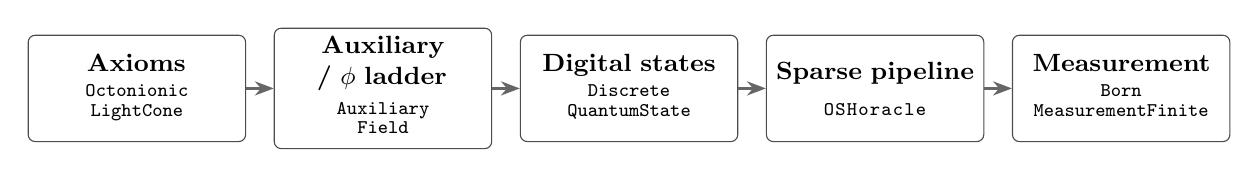
\begin{tikzpicture}[
  node distance=0.5cm and 0.35cm,
  box/.style={rectangle, draw=black!70, rounded corners=2.5pt, align=center, inner sep=3pt, minimum height=1.35cm, text width=2.55cm, font=\small},
  arr/.style={-{Stealth[length=2.4mm]}, thick, black!60}
]
\node[box] (ax) {\textbf{Axioms}\\[2pt]{\scriptsize\begin{tabular}{@{}c@{}}\lean{Octonionic}\\[-1pt]\lean{LightCone}\end{tabular}}};
\node[box, right=of ax] (aux) {\textbf{Auxiliary / }$\phi$\textbf{ ladder}\\[2pt]{\scriptsize\begin{tabular}{@{}c@{}}\lean{Auxiliary}\\[-1pt]\lean{Field}\end{tabular}}};
\node[box, right=of aux] (st) {\textbf{Digital states}\\[2pt]{\scriptsize\begin{tabular}{@{}c@{}}\lean{Discrete}\\[-1pt]\lean{QuantumState}\end{tabular}}};
\node[box, right=of st] (sp) {\textbf{Sparse pipeline}\\[2pt]{\scriptsize\lean{OSHoracle}}};
\node[box, right=of sp] (ms) {\textbf{Measurement}\\[2pt]{\scriptsize\begin{tabular}{@{}c@{}}\lean{Born}\\[-1pt]\lean{MeasurementFinite}\end{tabular}}};
\draw[arr] (ax) -- node[above, font=\scriptsize] {} (aux);
\draw[arr] (aux) -- (st);
\draw[arr] (st) -- (sp);
\draw[arr] (sp) -- (ms);
\end{tikzpicture}%
}
\caption{Lean-aligned pipeline (left to right). Variational layer: Section~\ref{sec:lagrangian}.}
\label{fig:roadmap}
\end{figure}

\section*{Acknowledgements}
The author acknowledges the use of AI-assisted development tools during manuscript and code production. In particular, Grok 4.20 and Composer 2 were used for programming assistance, Lean proof-development and verification support, and editorial revision support for manuscript drafting and refinement.

\section*{References}
\bibliographystyle{plain}
\bibliography{octonion_lightcone_to_oshoracle_refs}

\end{document}
